\newpage
\section{77. 组合}
\label{leetcode:77}

\subsection{题目}

给定两个整数 n 和 k,返回 \verb|1 ... n| 中所有可能的 k 个数的组合。

\textbf{示例}:

\begin{verbatim}
  输入: n = 4, k = 2
  输出:
  [
    [2,4],
    [3,4],
    [2,3],
    [1,2],
    [1,3],
    [1,4],
  ]
\end{verbatim}

\subsection{参考题解}

n = 4, k = 2 时状态树如下:

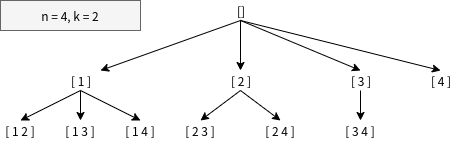
\includegraphics[width=100mm,height=50mm]{images/leetcode/leetcode_77.png}

n = 4, k = 3 时状态树如下:

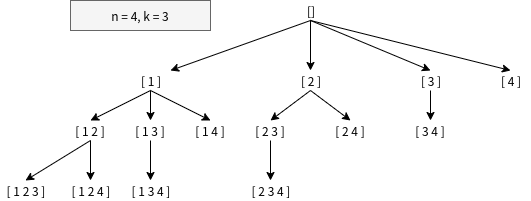
\includegraphics[width=100mm,height=50mm]{images/leetcode/leetcode_77_4_3.png}

遍历整个状态树,找到叶子节点中,数组长度等于 k 的节点,就是我们要的结果。

可以这么理解整个遍历的过程:

\begin{displaymath}
  \mathrm{C}_n^k = \mathrm{C}_{n-1}^{k-1} + \mathrm{C}_{n-1}^k
\end{displaymath}

$\mathrm{C}_n^k$ 表示在 n 个中取 k 个。
可以分为两种情况:

\begin{itemize}
  \item $\mathrm{C}_{n-1}^{k-1}$ 选择了第 n 个,然后我们只要在
    剩下的 n-1 个中选择 k-1 个。
  \item $\mathrm{C}_{n-1}^k$ 不选择第 n 个,那么我们需要在
    剩下的 n-1 个中选择 k 个。
\end{itemize}

\subsubsection{JavaScript}

\begin{verbatim}
/**
 * @param {number} n
 * @param {number} k
 * @return {number[][]}
 */
var combine = function(n, k) {
  let result = [];
  recursion(n, k, 1, [], result);
  return result;
};

function recursion(n, k, first, cur, result) {
  if (cur.length === k) {
    result.push(cur.slice())
    return;
  }

  for (let i = first; i <= n; i += 1) {
    cur.push(i);
    recursion(n, k, i + 1, cur, result);
    cur.pop();
  }
}
\end{verbatim}
